% Created 2022-04-11 Mon 12:21
% Intended LaTeX compiler: pdflatex
\documentclass[bigger]{beamer}
\usepackage[utf8]{inputenc}
\usepackage[T1]{fontenc}
\usepackage{graphicx}
\usepackage{grffile}
\usepackage{longtable}
\usepackage{wrapfig}
\usepackage{rotating}
\usepackage[normalem]{ulem}
\usepackage{amsmath}
\usepackage{textcomp}
\usepackage{amssymb}
\usepackage{capt-of}
\usepackage{hyperref}
\usetheme[progressbar=foot]{metropolis}
\author{Edmund Miller}
\date{2022-04-11 Mon}
\title{Nascent Transcript Identification}
\hypersetup{
 pdfauthor={Edmund Miller},
 pdftitle={Nascent Transcript Identification},
 pdfkeywords={},
 pdfsubject={},
 pdfcreator={Emacs 29.0.50 (Org mode 9.6)}, 
 pdflang={English}}
\makeatletter
\newcommand{\citeprocitem}[2]{\hyper@linkstart{cite}{citeproc_bib_item_#1}#2\hyper@linkend}
\makeatother

\usepackage[notquote]{hanging}
\begin{document}

\maketitle

\section*{Background}
\label{sec:org4d64b2c}
\section*{Gene Regulation}
\label{sec:org0a86e02}
\begin{frame}[label={sec:orgd44b062}]{Central Dogma of Biology}
\begin{center}
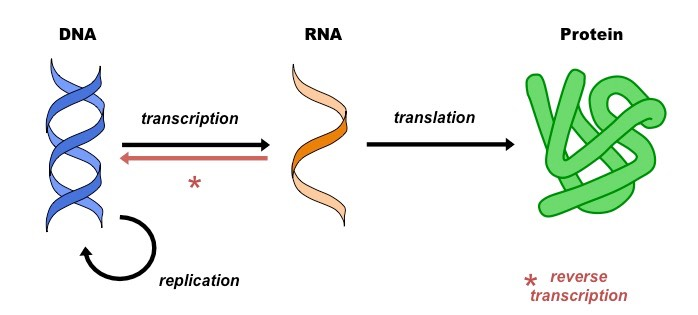
\includegraphics[width=.9\linewidth]{/home/emiller/src/personal/edmundmiller-dev/static/org-attach/b8/ce871b-5b7f-4cef-b389-7b27459818b3/_20220407_195627screenshot.png}
\end{center}
\end{frame}

\begin{frame}[label={sec:orgcc08c87}]{A Simple View of Gene Expression}
\begin{columns}
\begin{column}{0.45\columnwidth}
\begin{block}{Gene Expression}
\begin{center}
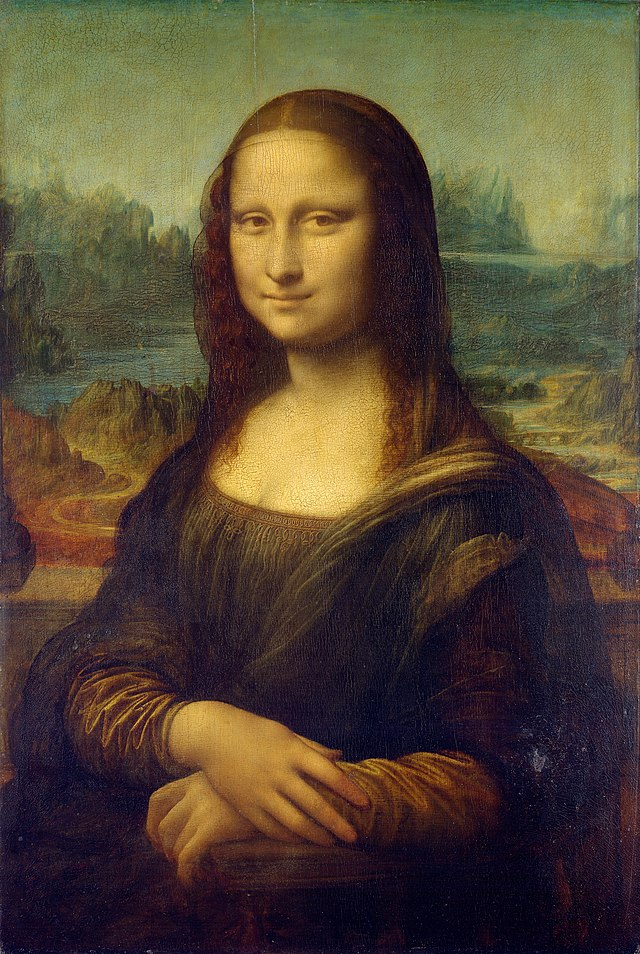
\includegraphics[width=.9\linewidth]{/home/emiller/src/personal/edmundmiller-dev/static/org-attach/a9/ae81d7-3773-4daa-baf6-bec17b6bb120/_20220407_195540screenshot.png}
\end{center}
\end{block}
\end{column}


\begin{column}{0.45\columnwidth}
\begin{block}{Central Dogma}
\begin{center}
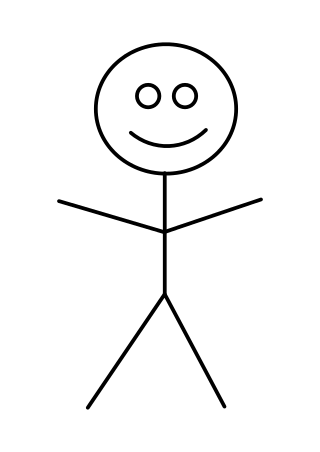
\includegraphics[width=.9\linewidth]{/home/emiller/src/personal/edmundmiller-dev/static/org-attach/a9/ae81d7-3773-4daa-baf6-bec17b6bb120/_20220407_195803screenshot.png}
\end{center}
\end{block}
\end{column}
\end{columns}
\end{frame}


\begin{frame}[label={sec:orgd6a45f1}]{Enhancers}
\begin{itemize}
\item Cis-acting DNA sequences that can increase the transcription of genes \footnote{(Pennacchio et al. 2013)\label{orge454700}}
\item The human genome contains hundreds of thousands of enhancers
\item Thought to work through DNA looping
\item Evidence of Enhancer-Promoter interaction from cross-linking assays(3c)
\end{itemize}
\end{frame}

\begin{frame}[label={sec:org91b676b}]{Topologically Associating Domain (TAD)}
\begin{figure}[htbp]
\centering
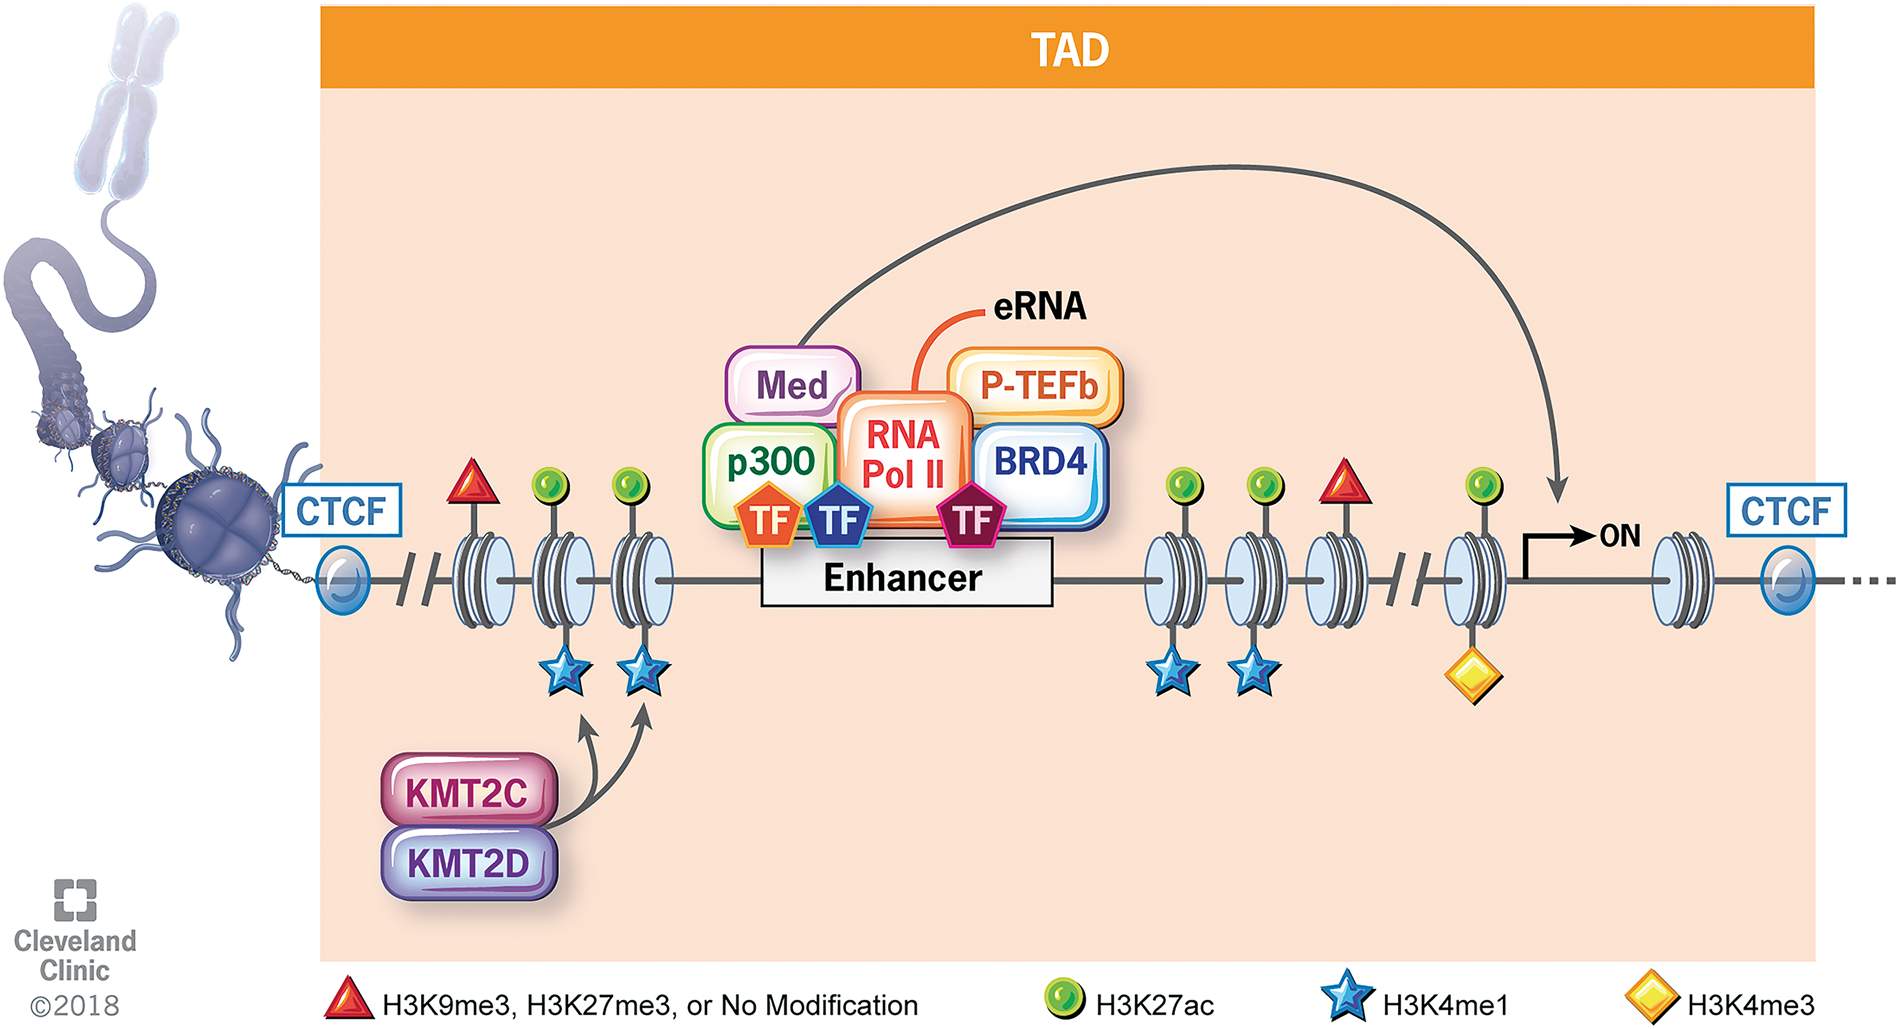
\includegraphics[width=.9\linewidth]{/home/emiller/src/personal/edmundmiller-dev/static/org-attach/5d/fc11b2-2dc8-4e7d-9034-57f92ff60114/_20220408_132400screenshot.png}
\caption{General topography of an active enhancer (Banerji, Rusconi, and Schaffner 1981).}
\end{figure}
\end{frame}

\begin{frame}[label={sec:org6f1dd46}]{Enhancer-promoter Looping}
\begin{figure}[htbp]
\centering
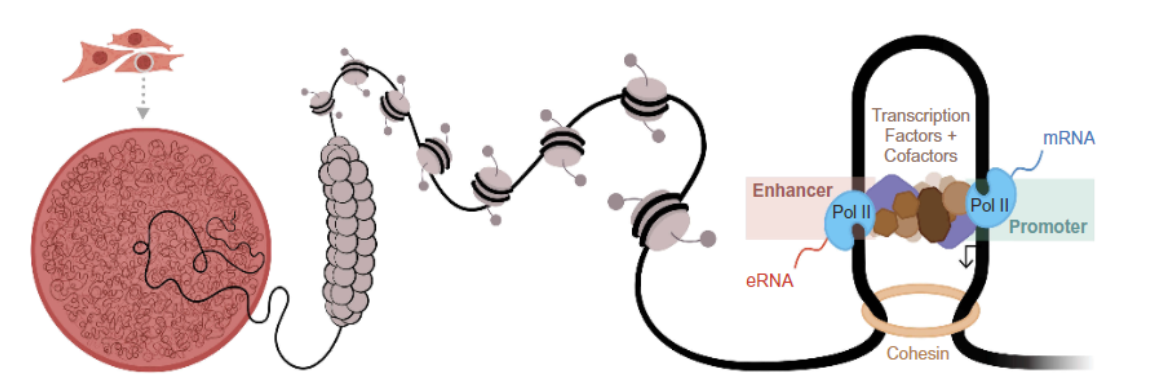
\includegraphics[width=.9\linewidth]{/home/emiller/src/personal/edmundmiller-dev/static/org-attach/1c/40bd96-7754-4e2b-9a2b-028570f5d89b/_20220408_144930screenshot.png}
\caption{(Murakami, Nagari, and Kraus 2017)}
\end{figure}
\end{frame}



\begin{frame}[label={sec:orga2e78cb}]{Why are Enhancers difficult to identify?}
\begin{enumerate}
\item Scattered across the 98\% of the human genome that does not encode proteins \textsuperscript{\ref{orge454700}}
\item Enhancers location relative to their target gene (or genes) is highly
variable. They can be upstream, downstream, or within introns. \textsuperscript{\ref{orge454700}}
\item Enhancers do not necessarily act on the respective closest promoter but can
bypass neighbouring genes to regulate genes located more distantly along a
chromosome \textsuperscript{\ref{orge454700}}
\end{enumerate}
\end{frame}

\begin{frame}[label={sec:org945ed36}]{Why are Enhancers difficult to identify?}
\begin{enumerate}
\item One Enhancer can regulate multiple genes \footnote{(Mohrs et al. 2001)} and One
gene can be regulated by multiple enhancers \footnote{(Kim et al. 2018)}
\item The general sequence code of enhancers, if one exists at all, is poorly
understood. \textsuperscript{\ref{orge454700}}
\item The activity of enhancers can be restricted to a particular tissue or cell type
\end{enumerate}
\end{frame}

\begin{frame}[label={sec:orgae6d45f}]{Multiple Enhancers can regulate one gene}
\begin{figure}[htbp]
\centering
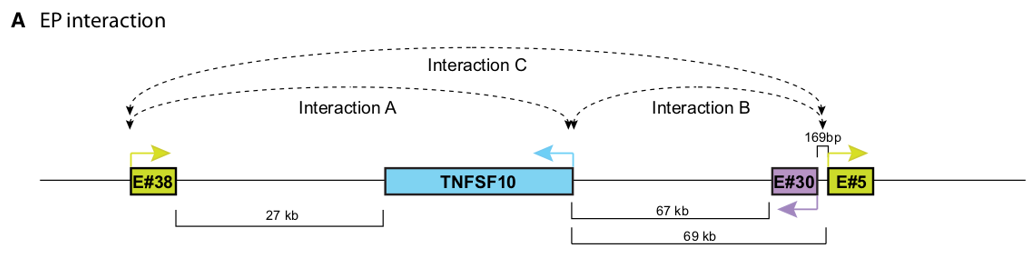
\includegraphics[width=.9\linewidth]{/home/emiller/src/personal/edmundmiller-dev/static/org-attach/41/914259-ccb3-42b6-a38e-7e284c0bdded/_20220408_094258screenshot.png}
\caption[Short caption]{(Kim et al. 2018)}
\end{figure}
\end{frame}


\begin{frame}[label={sec:orgc7fde44}]{eRNAs Introduction}
\begin{itemize}
\item Sense and antisense transcripts from enhancers
\item Play a role in the activation because the knockdown of a subset of the eRNAs
resulted in decreased gene transcription \footnote{(Ulf Andersson Ørom 2010)}
\item Used to identify active enhancers
\end{itemize}
\end{frame}

\section*{Global Transcriptional Activity Dynamics Reveal Functional Enhancer RNAs}
\label{sec:org7007425}
\begin{frame}[label={sec:org992b822}]{Global Transcriptional Activity Dynamics Reveal Functional Enhancer RNAs}
\begin{center}
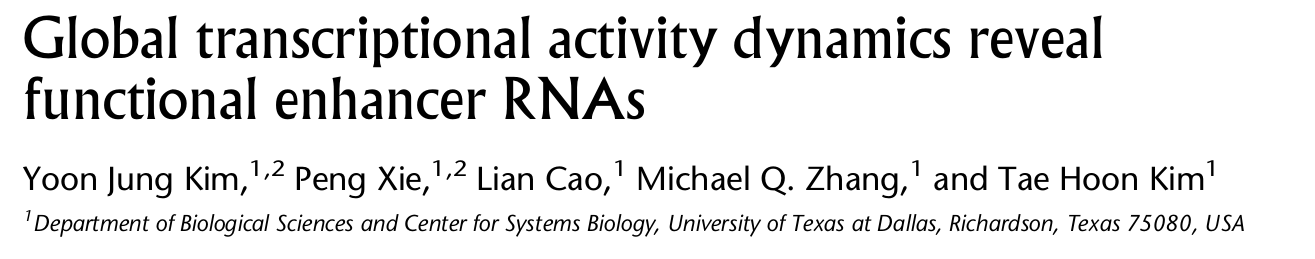
\includegraphics[width=.9\linewidth]{/home/emiller/src/personal/edmundmiller-dev/static/org-attach/d2/b368ba-de24-48ff-a497-6012a72fd306/_20220408_195834screenshot.png}
\end{center}
\end{frame}

\begin{frame}[label={sec:org5af570a}]{GRO-Seq Overview}
\begin{center}
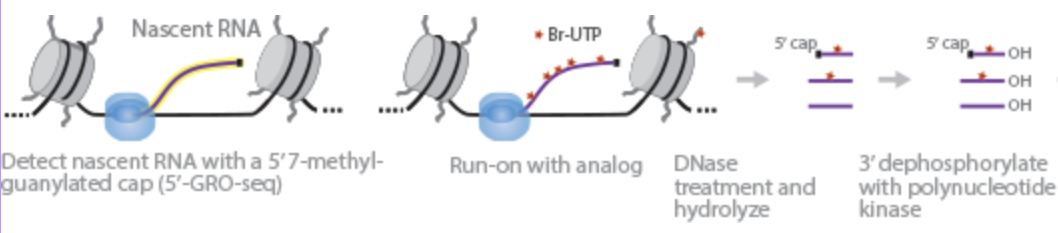
\includegraphics[height=0.18\linewidth]{/home/emiller/src/personal/edmundmiller-dev/static/org-attach/08/136bc2-5fce-4dbb-bdb3-14793c5261d3/_20220411_121046screenshot.png}
\end{center}

\begin{figure}[htbp]
\centering
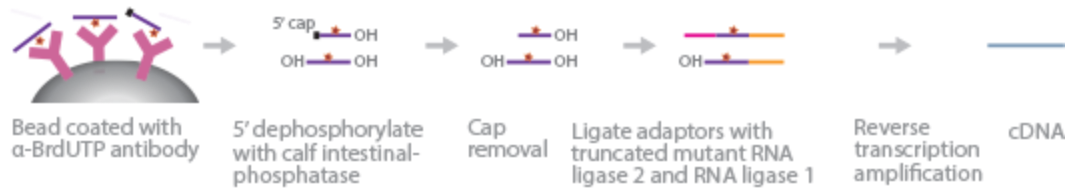
\includegraphics[height=0.18\linewidth]{/home/emiller/src/personal/edmundmiller-dev/static/org-attach/08/136bc2-5fce-4dbb-bdb3-14793c5261d3/_20220411_121114screenshot.png}
\caption{\href{https://www.illumina.com/science/sequencing-method-explorer/kits-and-arrays/5--gro-seq.html}{Illumina Sequencing Methods}}
\end{figure}
\end{frame}


\begin{frame}[label={sec:orgb392d6a}]{GRO-Seq pros and cons}
\begin{block}{Pros:}
\begin{itemize}
\item Maps nascent capped 5' RNA sequence at any given time
\item Determines activity of transcription sites
\item No prior knowledge of transcription sites needed
\end{itemize}
\end{block}

\begin{block}{Cons:}
\begin{itemize}
\item Limited to cell cultures and other artificial systems due to incubation with
labelled nucleotides
\end{itemize}
\end{block}
\end{frame}

\begin{frame}[label={sec:org0babe6b}]{Kim et. al 2018 Summary}
\begin{figure}[htbp]
\centering
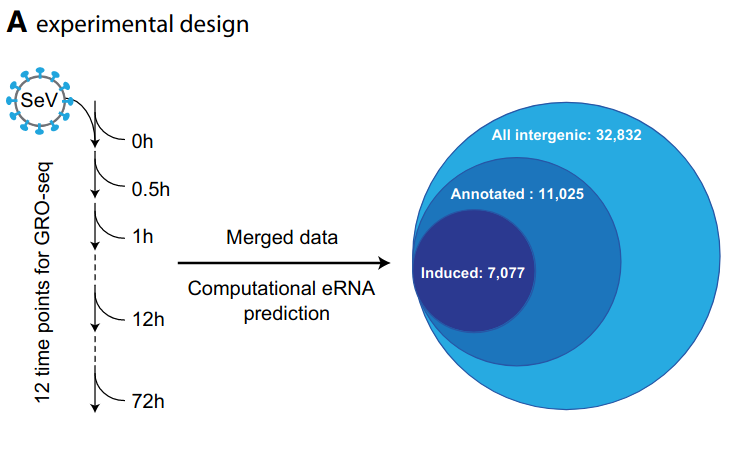
\includegraphics[width=.9\linewidth]{/home/emiller/src/personal/edmundmiller-dev/static/org-attach/38/cec5e3-c50e-4d76-9126-cf4883249f97/_20220411_101902screenshot.png}
\caption[Short caption]{(Kim et al. 2018)}
\end{figure}
\end{frame}


\begin{frame}[label={sec:orgd7865a3}]{Kim et. al 2018 Summary}
\begin{center}
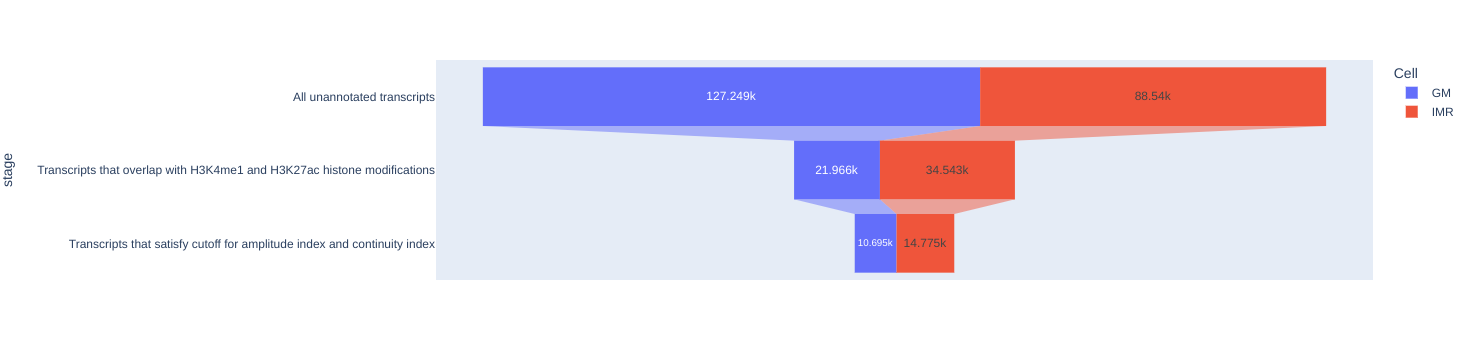
\includegraphics[height=0.25\linewidth]{/home/emiller/src/personal/edmundmiller-dev/static/org-attach/75/4a799c-2e12-4613-9543-8d4311f83462/newplot.png}
\end{center}
\end{frame}

\begin{frame}[label={sec:orgab3f8cc}]{Kim et. al 2018 Summary}
\begin{figure}[htbp]
\centering
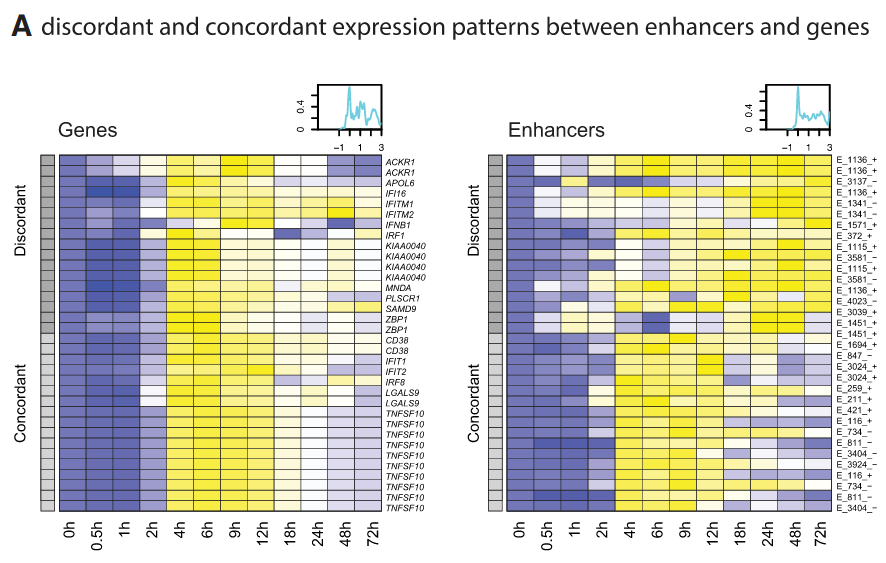
\includegraphics[width=.9\linewidth]{/home/emiller/src/personal/edmundmiller-dev/static/org-attach/fa/b0e52a-4588-4f5b-a045-debb7f415eeb/_20220411_102139screenshot.png}
\caption[Short caption]{(Kim et al. 2018)}
\end{figure}
\end{frame}



\begin{frame}[label={sec:org31dd82c}]{Kim et. al 2018 Summary}
\begin{figure}[htbp]
\centering
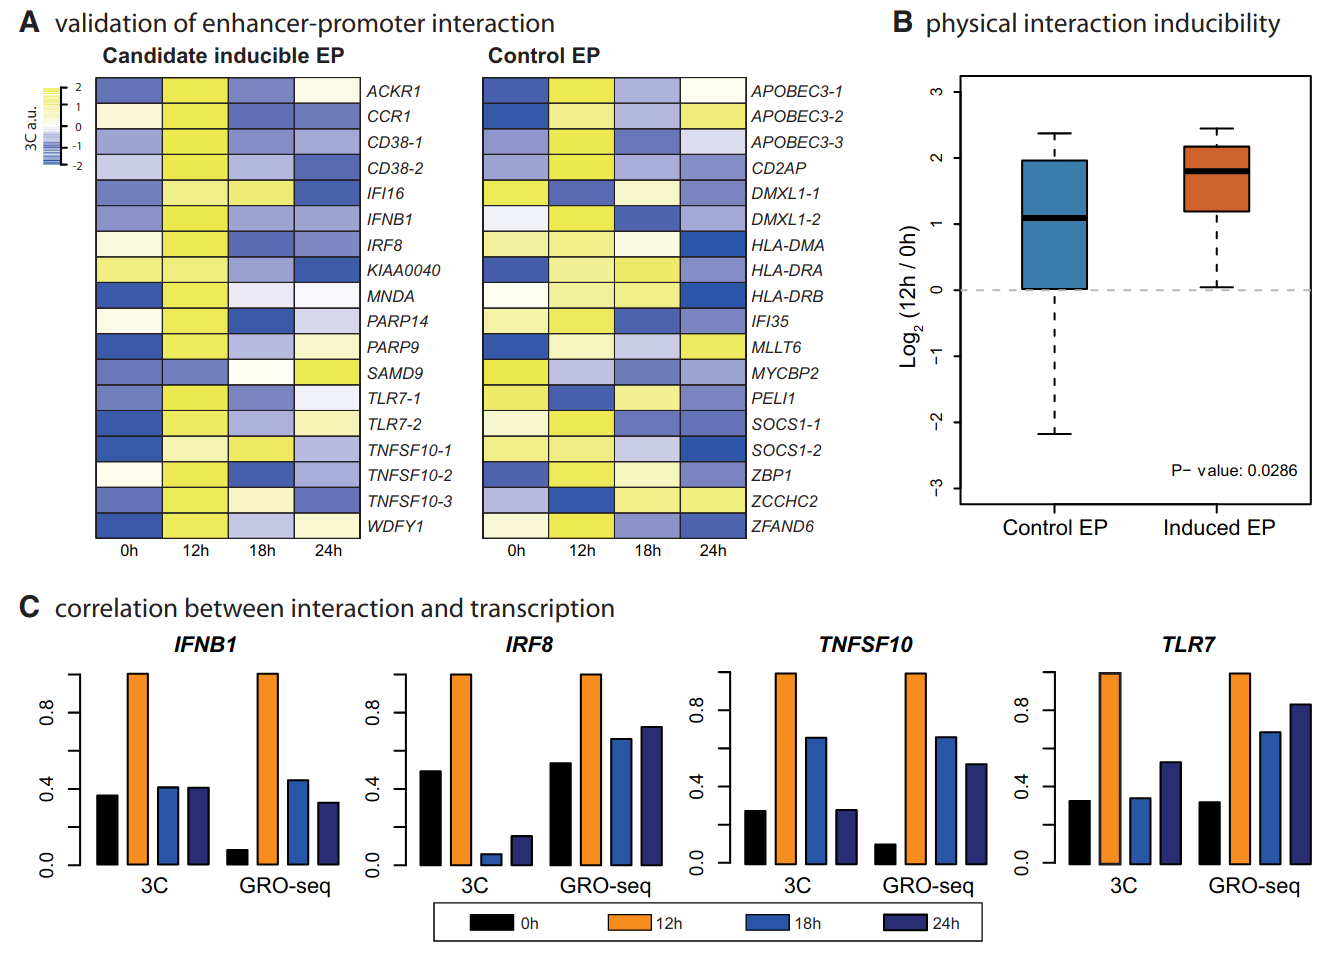
\includegraphics[width=.9\linewidth]{/home/emiller/src/personal/edmundmiller-dev/static/org-attach/28/c3910e-fa74-4824-a617-3598712149e4/_20220411_102205screenshot.png}
\caption[Short caption]{(Kim et al. 2018)}
\end{figure}
\end{frame}

\begin{frame}[label={sec:orgd236887}]{Reproduction with Parallel IMR Dataset}
\begin{itemize}
\item Wrote workflow using snakemake
\item Goal was to reproduce GM results
\item Achieved \alert{80\%} of predicted eRNAs due to difficulty with nascent transcript
identification
\end{itemize}
\end{frame}

\begin{frame}[label={sec:org5ba254e}]{Hypothesis}
\begin{itemize}
\item Does the standardization of secondary analysis and use of transcription start
sites for calling enhancer RNAs improve the accuracy full transcript
identification?
\item Using the streamlined process of transcript identification can new dynamics
and classes of eRNAs can be indentified from massively parrallel processing of
publicly accessible nascent trancript assay across cell lines?
\end{itemize}
\end{frame}
\section*{Aims}
\label{sec:org9eff12c}
\section*{Aim 1: Create a best practice secondary analysis pipeline for nascent transcripts}
\label{sec:org25732fe}
\begin{frame}[label={sec:org061865d}]{Standardizing Snakemake Workflow}
\begin{itemize}
\item January 2020
\item Template
\item Universal Commands
\item Testing
\item CI/CD
\item Wrappers
\end{itemize}
\end{frame}

\begin{frame}[label={sec:org87c7727}]{nf-core Paper}
\begin{center}
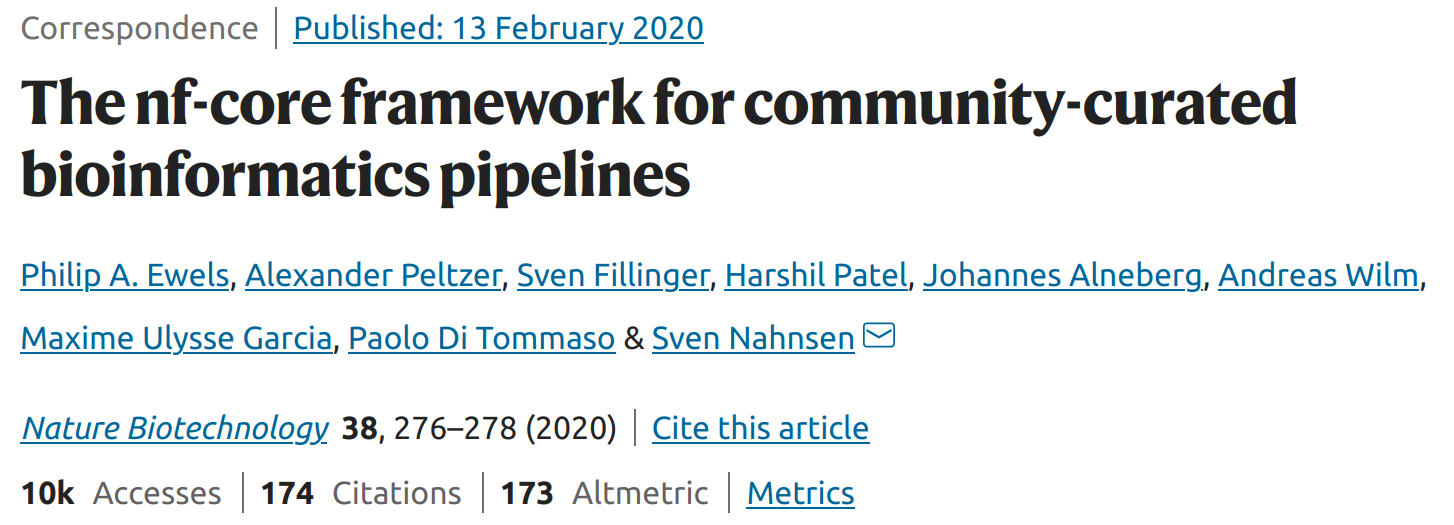
\includegraphics[width=.9\linewidth]{/home/emiller/src/personal/edmundmiller-dev/static/org-attach/44/19713d-e23c-403b-b4e2-0c30201bfbac/_20220411_115734screenshot.png}
\end{center}
\end{frame}

\begin{frame}[label={sec:org99708cc}]{Main concepts of nf-core}
\begin{figure}[htbp]
\centering

\includegraphics[height=0.6\linewidth]{/home/emiller/src/personal/edmundmiller-dev/static/org-attach/b9/be7b67-b57f-4f58-8cda-36455fb83c53/_20220411_115958screenshot.png}
\caption{(Ewels et al. 2020)}
\end{figure}
\end{frame}




\begin{frame}[label={sec:org9a49b32},fragile]{nf-core Getting started}
 \begin{verbatim}
# Install nextflow
curl -s https://get.nextflow.io | bash
mv nextflow ~/bin/

# Launch the Nascent pipeline
nextflow run nf-core/nascent \
    --input samplesheet.csv \
    --genome GRCh38 \
    -profile docker
\end{verbatim}
\end{frame}

\begin{frame}[label={sec:org5f293f7}]{Inheriting nf-core Nascent}
\begin{itemize}
\item Breaking our analysis up into smaller pieces
\item nf-core portion includes Quality Checks, alignment, graph generation, transcript
identification, and transcript quantification
\item Downstream analysis is then a seperate nextflow workflow
\item Data engineering/Data Science split
\end{itemize}
\end{frame}

\begin{frame}[label={sec:org151f3aa}]{Primary-Secondary-Tertiary Analysis}
\begin{center}
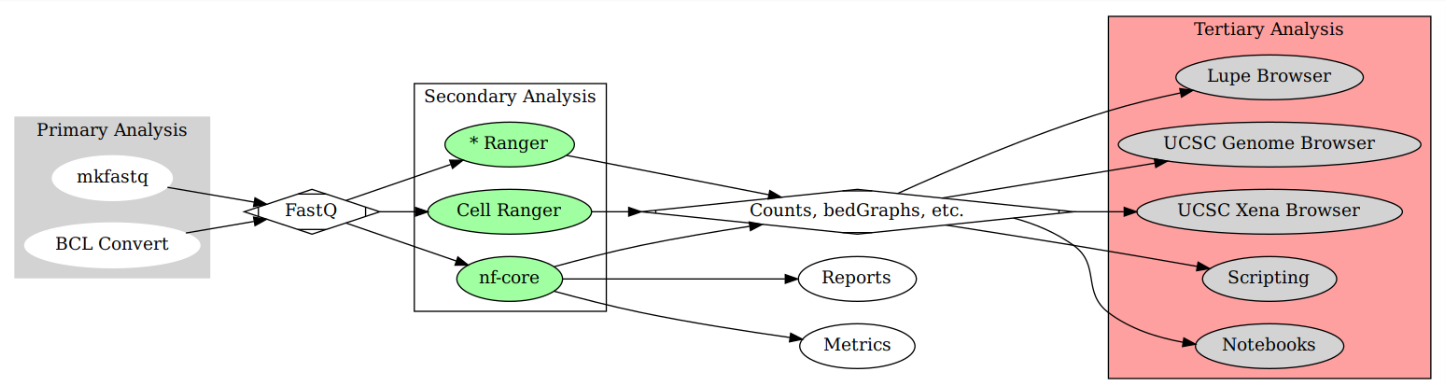
\includegraphics[width=.9\linewidth]{/home/emiller/src/personal/edmundmiller-dev/static/org-attach/31/b1315d-d636-4cd7-928c-db5f94855d6f/_20220411_104006screenshot.png}
\end{center}
\end{frame}

\begin{frame}[label={sec:orgb93af4b}]{Nascent Goals}
\begin{itemize}
\item Benchmark aligners to find best practices(Lots of opinions, no hard numbers)
\item Handle alignment, QC, Genome graph generation, and naive transcript
identification
\end{itemize}
\end{frame}

\section*{Aim 2: Take advantage of New Developments to improve eRNA annotation}
\label{sec:orgee4e2df}
\begin{frame}[label={sec:orgf08ce5f}]{New developments}
\begin{itemize}
\item CHM13 Released
\item PINTS and transcriptional regulatory elements (TREs) matrix
\end{itemize}
\end{frame}

\begin{frame}[label={sec:org1a0363b}]{CHM13}
\begin{figure}[htbp]
\centering
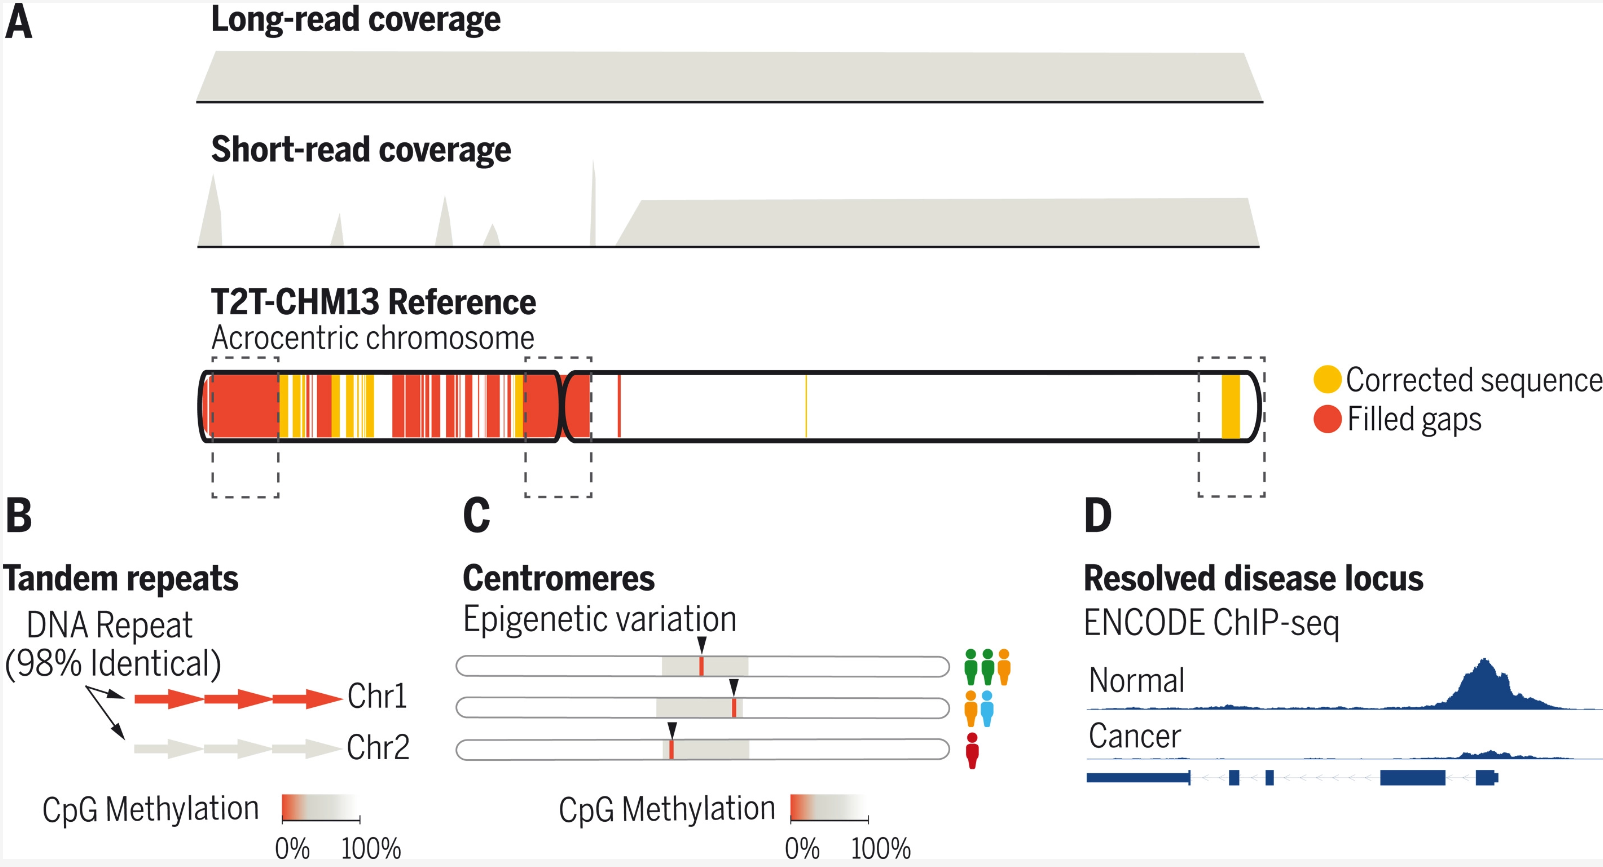
\includegraphics[width=.9\linewidth]{/home/emiller/src/personal/edmundmiller-dev/static/org-attach/80/87b00d-bcee-415d-99c3-34afae64e91a/_20220411_101653screenshot.png}
\caption{(Gershman et al. 2022)}
\end{figure}
\end{frame}

\begin{frame}[label={sec:org95a07aa}]{CHM13}
\begin{figure}[htbp]
\centering
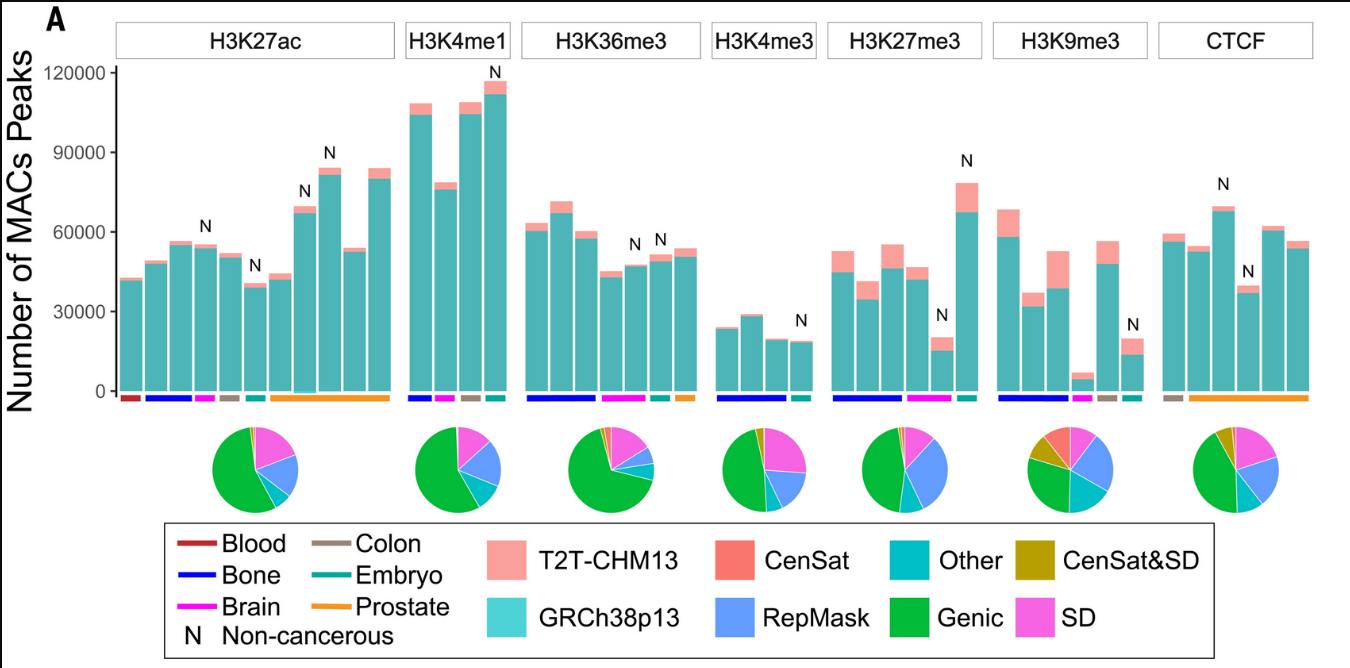
\includegraphics[width=.9\linewidth]{/home/emiller/src/personal/edmundmiller-dev/static/org-attach/82/69b2b8-4cb6-4bf3-a0c1-3604fdd4d423/_20220411_101552screenshot.png}
\caption{(Gershman et al. 2022)}
\end{figure}
\end{frame}



\begin{frame}[label={sec:org65af9fa}]{PINTS - different patterns of signals captured by TSS and NT Assays}
\begin{figure}[htbp]
\centering
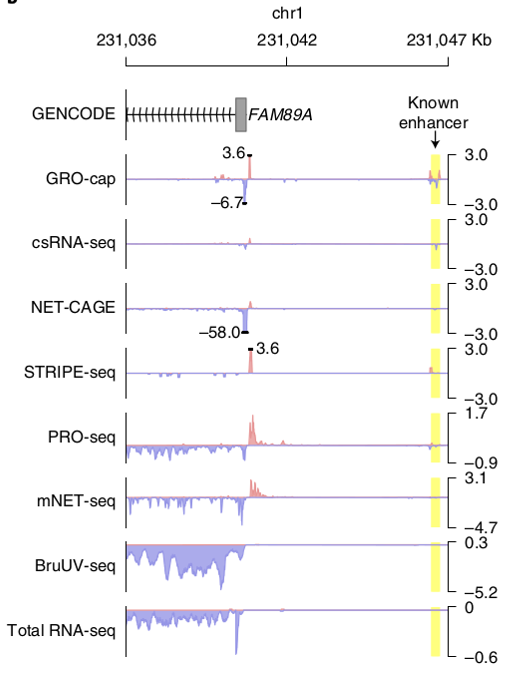
\includegraphics[height=0.6\linewidth]{/home/emiller/src/personal/edmundmiller-dev/static/org-attach/48/3e1795-ac17-4e6b-a14b-37222b74a24d/_20220411_103318screenshot.png}
\caption{(Yao et al. 2022)}
\end{figure}
\end{frame}


\begin{frame}[label={sec:org1acedfe}]{PINTS - NT vs TSS assays}
\begin{figure}[htbp]
\centering
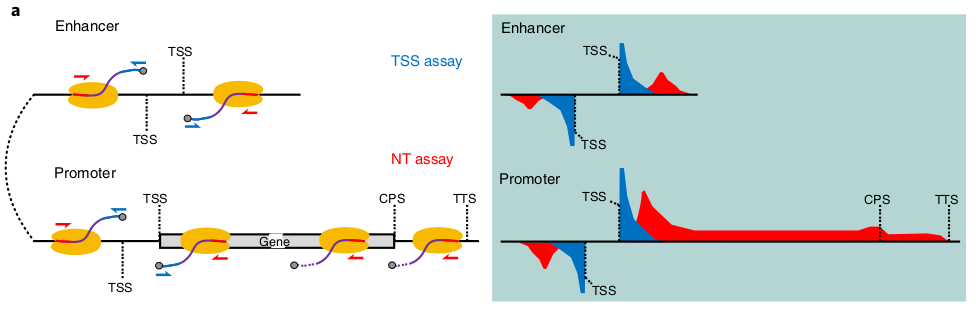
\includegraphics[height=0.35\linewidth]{/home/emiller/src/personal/edmundmiller-dev/static/org-attach/cb/525ffe-5925-48af-a434-cff675b835be/_20220408_112049screenshot.png}
\caption{(Yao et al. 2022)}
\end{figure}
\end{frame}

\begin{frame}[label={sec:org21664d2}]{PINTS}
\begin{figure}[htbp]
\centering
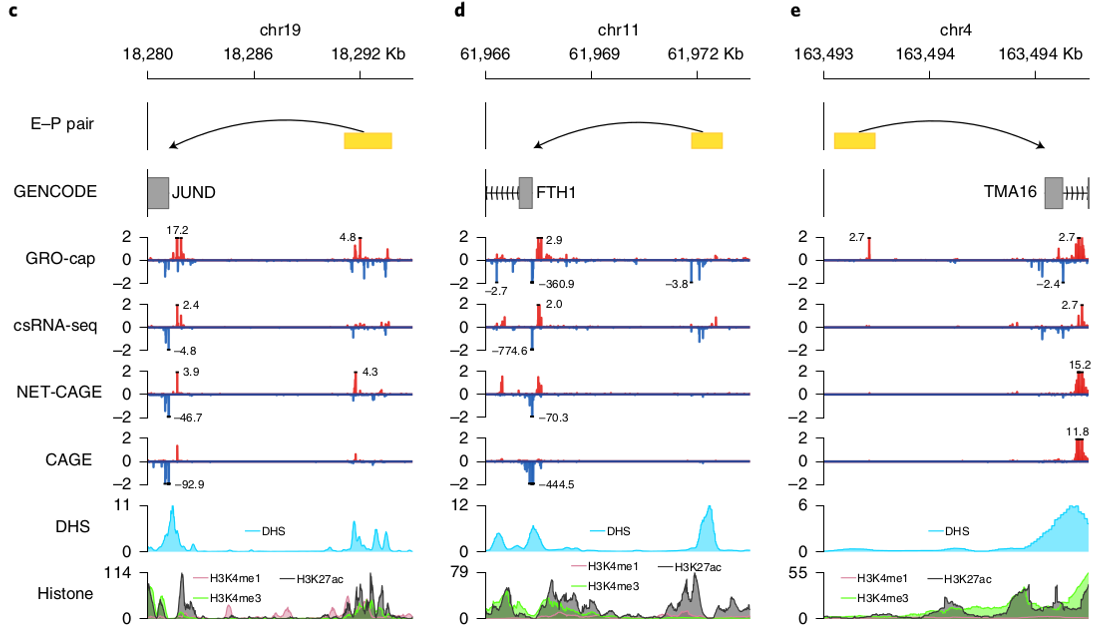
\includegraphics[width=.9\linewidth]{/home/emiller/src/personal/edmundmiller-dev/static/org-attach/47/b91df4-1791-4121-9c6c-ee1c403115b1/_20220411_103434screenshot.png}
\caption{(Yao et al. 2022)}
\end{figure}
\end{frame}


\begin{frame}[label={sec:orga438979}]{PINTS}
\begin{itemize}
\item Can we use PINTS for Nascent Transcript Assays?
\item Can we swap naive method of selecting for Histone modications with PINTS
indentified transcriptional regulatory elements (TREs)?
\item Can we indetify full length transcripts from the Nascent Transcript assays?
\end{itemize}
\end{frame}

\section*{Aim 3 Compare eRNA dynamics between cell lines}
\label{sec:org757c2b1}
\begin{frame}[label={sec:orgbf2fdfe}]{IMR and GM}
\begin{itemize}
\item GM12878 - lymphoblastoid(immune response) cell line produced from the blood of
a female donor (ENCODE Tier 1)
\item IMR90 - fibroblasts(connective tissue) isolated from the normal lung
tissue(ENCODE Tier 2.5)
\end{itemize}
\end{frame}

\begin{frame}[label={sec:org2c4b34f}]{IMR and GM}
\begin{center}
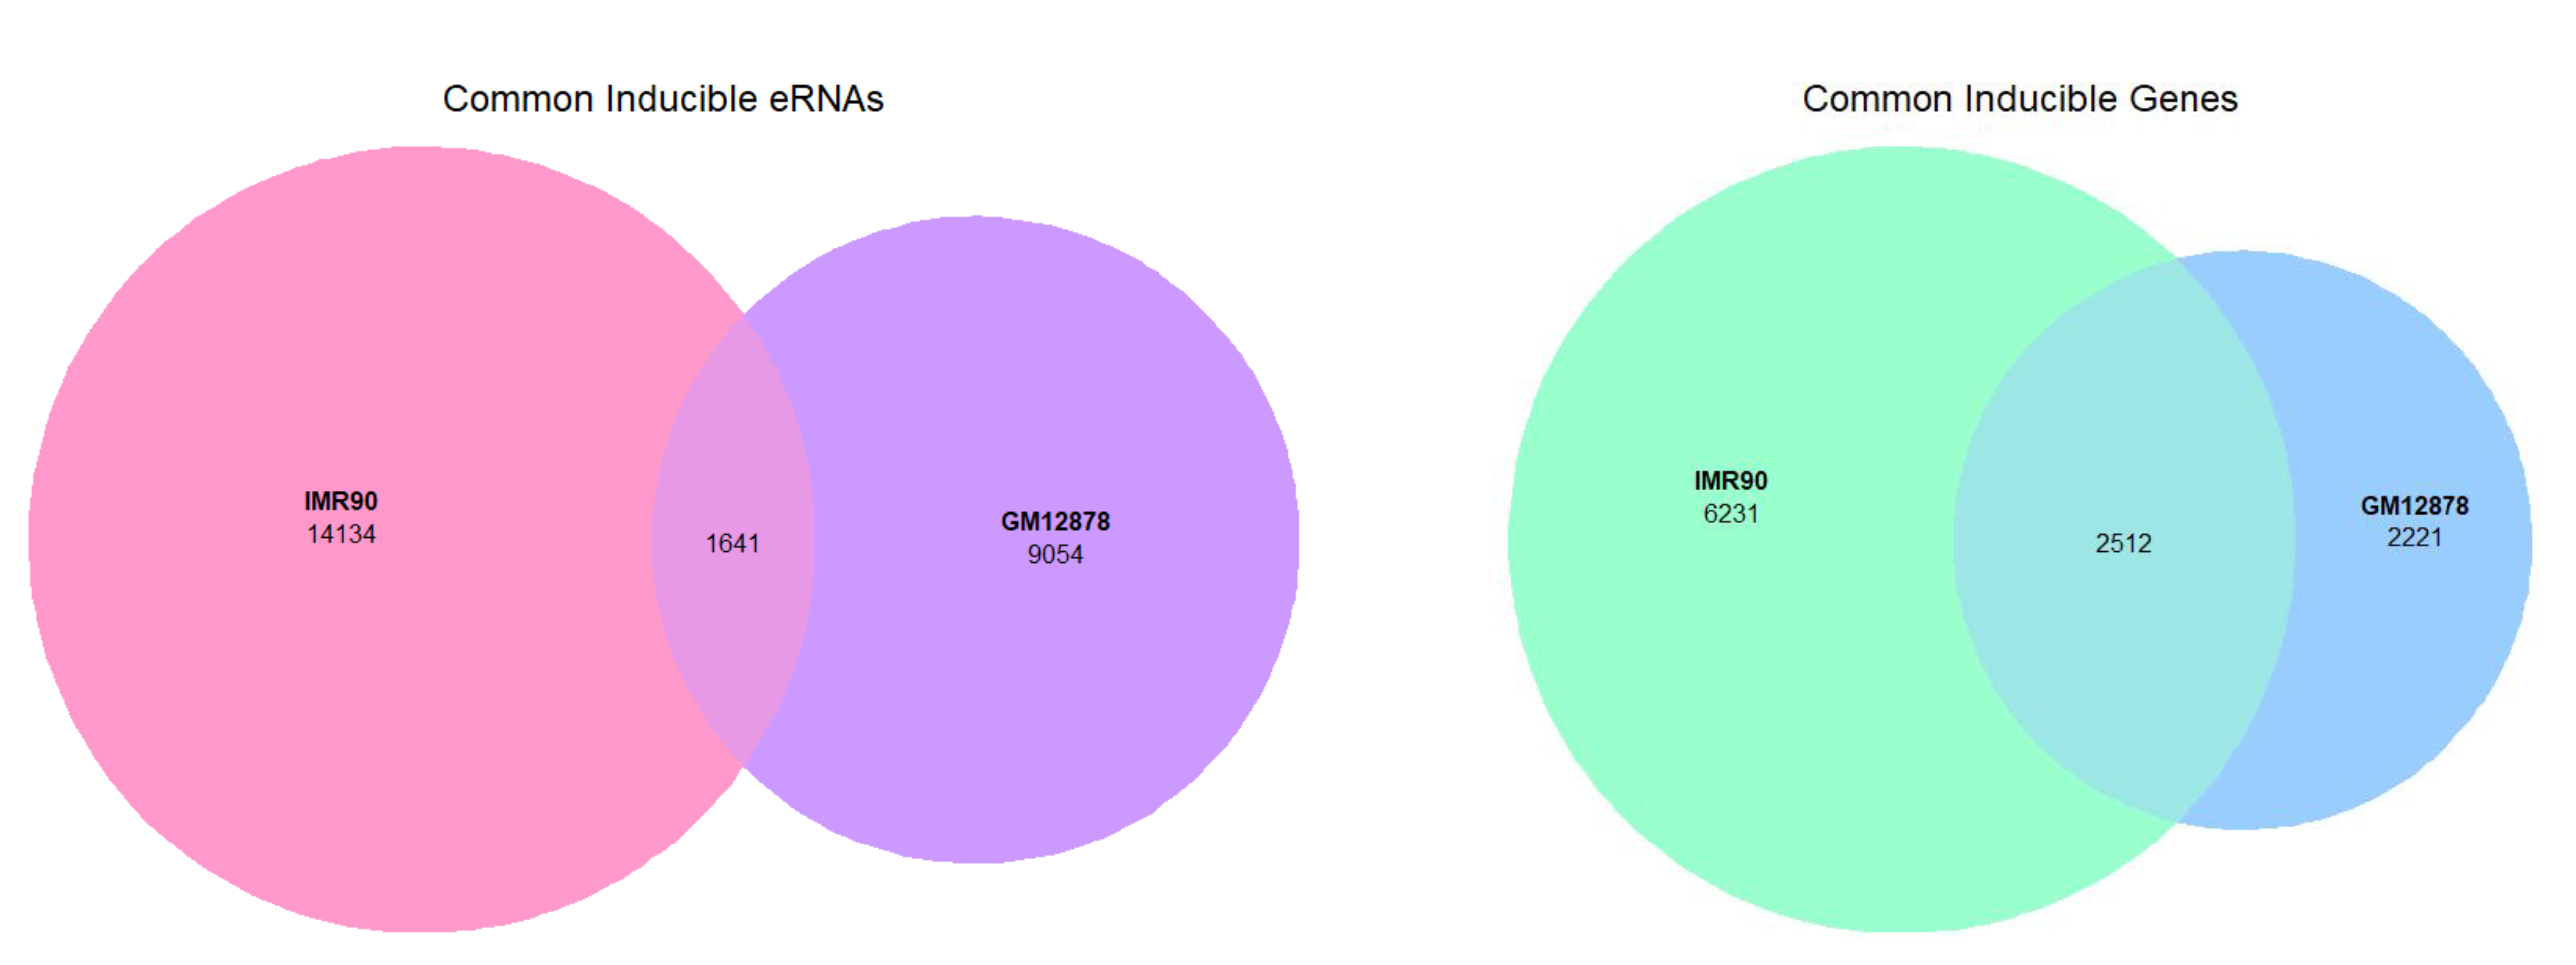
\includegraphics[width=.9\linewidth]{/home/emiller/src/personal/edmundmiller-dev/static/org-attach/75/69a87c-da73-4704-a6b9-86b1ca1150d4/_20220411_105101screenshot.png}
\end{center}
\end{frame}
\begin{frame}[label={sec:orgef26d4e}]{Cell-Type Specific eRNAs}
\begin{center}
\begin{tabular}{lr}
Common inducible genes: & 2512\\
Common inducible genes with cell-type specific eRNAs: & 2053\\
\end{tabular}
\end{center}

\begin{itemize}
\item 81.7\%  Common inducible genes had \alert{cell-type} specific eRNAs
\item While they may have a common gene expression each cell line had their own
unique way of solving the need.
\end{itemize}
\end{frame}
\end{document}
